\documentclass[journal, onecolumn]{IEEEtran}

\usepackage{amsmath, amsfonts, amssymb}
\usepackage{hyperref}
\usepackage[final]{graphicx}

\begin{document}

\title{Preprocessing Methodology for Archaic Modi Script Translation}
\author{}
\maketitle

\section{Overview}
Preprocessing acts as a foundational, critical mechanism within the broader architecture of translating historical documents. Given that archival manuscripts natively suffer from acute degradation, fading, and physical damage spanning centuries, raw imaging data contains vast quantities of visual noise. The primary role of the preprocessing pipeline is to aggressively isolate the target handwritten manuscript ink from complex backgrounds. By standardizing the continuous visual inputs into high-contrast morphological structures, the pipeline fundamentally reduces the latent variance that downstream Vision-Language Models must account for, directly improving their capacity to learn accurate transliteration mappings.

\section{Previous Research and Methodological Novelty}
The foundational dataset and baseline Vision-Language Model (VLM) framework for the transliteration of Modi script to Devanagari were introduced by Kausadikar et al. \cite{kausadikar2026}. While their work provided the critical raw document image dataset essential for this domain, their preprocessing methodology fundamentally lacked advanced topological filtering. Consequently, the baseline images processed in their framework suffered from residual speckles, ink-bleed artifacts, and noise clusters that resemble valid Modi characters, which inherently degrades VLM character recognition performance. 

Our preprocessing pipeline introduces a significant novelty by integrating aggressive, geometrically bounded speckle and artifact removal heuristics. By coupling adaptive binarization with a strictly constrained Connected Components analysis, our approach explicitly isolates true graphemic structures, completely extinguishing the historical paper noise that was previously passed into the baseline models.

\section{Dataset Description (Pre-Preprocessing Context)}
The raw dataset consists of continuous-tone digital captures of historical manuscripts written in the cursive, continuous Modi script. These documents, sourced primarily from governmental and historical archives, are characterized by severe physical and temporal degradation. Native characteristics include damp patches, fading ink, paper browning (foxing), ink bleed-through from the reverse sides of pages, script fragmentation, and extensive non-uniform illumination due to varied digitization conditions. The data is initially provided in multi-band Red-Green-Blue formats.

\section{Step-by-Step Preprocessing Techniques}

\subsection{Grayscale Conversion}
The initial stage of the pipeline transforms the multiband color image into a single-channel intensity image. By computing the weighted sum of color channels according to human perceptual luminances, we establish a standardized intensity map. This technique is computationally vital as the chromatic information in monochrome manuscript inks is largely redundant for structural decipherment. It dramatically accelerates subsequent processing stages by reducing dimensionality. The assumption is that the distinction between ink and paper background relies purely on relative intensity rather than hue.

Its mathematical formulation is defined as:
\begin{equation}
Y = 0.299R + 0.587G + 0.114B
\end{equation}

\subsection{Edge-Preserving Denoising (Bilateral Filtering)}
To mitigate native paper textures and sensor noise without blurring the sharp stroke boundaries of the handwritten script, a non-linear bilateral filter is applied \cite{tomasi1998}. Unlike standard Gaussian blurs, the bilateral filter utilizes both spatial proximity and intensity proximity to calculate average values. This technique is justified because historical documents contain high-frequency noise distributed across low-frequency background patches, coupled with high-frequency ink boundaries that absolutely must be preserved for accurate morphological extraction. It assumes that ink boundaries present a sharper intensity gradient than surrounding noise.

Its mathematical formulation at a given spatial location is:
\begin{equation}
I^{filtered}(x) = \frac{1}{W_p} \sum_{x_i \in \Omega} I(x_i) \cdot f_r(\|I(x_i) - I(x)\|) \cdot g_s(\|x_i - x\|)
\end{equation}
Where $W_p$ is the normalization factor, $f_r$ is the intensity range kernel, and $g_s$ is the spatial domain kernel.

\subsection{Adaptive Gaussian Thresholding}
Global thresholding algorithms routinely fail on archival documents due to illumination gradients spanning the page. Adaptive Gaussian Thresholding \cite{bradley2007} resolves this by binarizing the image using a localized, dynamic threshold calculated over a highly specific pixel radius. This is critically justified as it normalizes dynamic lighting conditions, extracting faint text located in dark corners just as efficiently as bold text under bright illumination. It assumes that within any localized spatial block, there exists sufficient variance to calculate an accurate binarization threshold separating paper from ink.

Its mathematical formulation computes the local threshold and the corresponding mask:
\begin{equation}
T(x, y) = \text{GaussianWeight}(x, y) * I_{window} - C
\end{equation}
\begin{equation}
I^{binary}(x, y) = \begin{cases} 255, & \text{if } I(x, y) > T(x, y) \\ 0, & \text{otherwise} \end{cases}
\end{equation}

\subsection{Speckle and Artifact Removal via Connected Components}
Unlike the baseline approach described by Kausadikar et al. \cite{kausadikar2026}, which relied on standard binarization leaving noisy remnants, our pipeline aggressively identifies and eliminates minute, disconnected dots caused by aged-paper artifacts or local binarization failures over stains. A Connected Components Analysis assesses the structural mass of contiguous pixels. Components failing to satisfy bounded minimum dimensional limits are computationally erased from the foreground mask. Given the cursive, continuous flow inherent to the Modi script, legitimate strokes present significant pixel counts and structural dimensions. Removing isolated pixel clusters forces the network to focus strictly on genuine graphemes rather than paper grain. This mathematically assumes that script ink guarantees an identifiable spatial mass exceeding basic thresholds.

Its mathematical formulation defines a preserved component belonging to the set of all objects $\mathcal{C}$ subject to dimensional evaluations:
\begin{equation}
\text{Keep}(c) = \text{Area}(c) \geq \tau_{area} \lor (\text{Height}(c) \geq \tau_{h} \land \text{Width}(c) \geq \tau_{w})
\end{equation}

To demonstrate the crucial necessity and empirical superiority of this novel speckle removal strategy, Figure \ref{fig:speckle_comparison} presents a direct structural comparison. The raw sample is utilized from the dataset developed by \cite{kausadikar2026}.

\begin{figure}[htbp]
\centering
\begin{minipage}{0.48\textwidth}
\centering
% Add your image here: 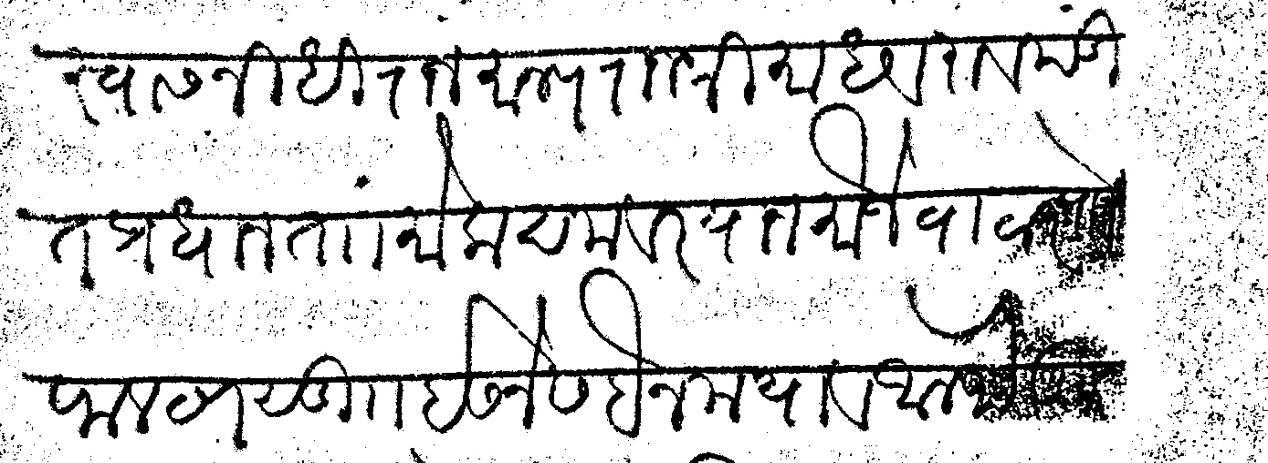
\includegraphics[width=\linewidth]{images_raw/example5.jpg}
\vspace{6cm} % Blank placeholder space
\caption{Raw Modi script sample from the dataset introduced by Kausadikar et al. \cite{kausadikar2026}, exhibiting heavy background artifacts.}
\end{minipage}\hfill
\begin{minipage}{0.48\textwidth}
\centering
% Add your image here: \includegraphics[width=\linewidth]{images_preprocessed/example5_preprocessed.png}
\vspace{6cm} % Blank placeholder space
\caption{Our proposed output highlighting absolute speckle removal and isolated grapheme extraction.}
\label{fig:speckle_comparison}
\end{minipage}
\end{figure}

\subsection{False-Positive Foreground Suppression}
Adaptive binarization algorithms frequently over-compensate, occasionally forcing heavy background stains into solid foreground objects. To suppress these false positives, the remaining component masks are juxtaposed against the original grayscale matrix to evaluate their underlying mean intensity. Background noise mapped as text frequently possesses a much lighter true intensity than actual carbon-based ink. Extinguishing components that fail this severity check ensures that margin stains are not passed into the vision encoder. The assumption holds that true ink strokes universally represent the darkest absolute values across the historic document.

Its mathematical formulation validates an extracted mask component cluster $M_c$:
\begin{equation}
\frac{1}{|M_c|} \sum_{(x,y) \in M_c} I^{gray}(x,y) \leq \tau_{ink}
\end{equation}

\subsection{Deskewing}
To optimize the alignment of textual baselines for the neural network, the skew angle of the general foreground text can be calculated via minimum area bounding rectangles, followed by an affine rotation sequence. While theoretically pertinent for reducing spatial variance, deskewing is intentionally bypassed in the current highly-fragmented archival pipeline to circumvent catastrophic over-rotations fundamentally triggered by noise matrices sitting on the extremities of fragmented documents.

\section{Algorithmic and Implementation Details}
The preprocessing pipeline is exclusively engineered inside Python 3, capitalizing on the OpenCV library for extremely efficient low-level C++ matrix operations and NumPy for rapid vectorized array evaluations. The bilateral filter implements a kernel diameter of 5 with substantial color and spatial sigma parameters rated at 100, effectively demanding aggressive smoothing while harshly terminating at stroke boundaries. The adaptive thresholding leverages a massive block dimension of 61 accompanied by a subtractive constant of 21, specifically scaled to accommodate high-resolution scans while filtering illumination sweeps. Geometric component filters impose firm base constraints demanding an area minimum of 100 pixels alongside rigid height and width metrics. Ultimately, the ink intensity suppressor imposes a strict cap of 130 on the 8-bit scale, eradicating lighter false-positives globally.

\section{Impact on Model Performance}
Applying this preprocessing configuration substantially optimizes downstream modeling efforts. By explicitly terminating severe historical noise arrays and illuminating only structural strokes, the Vision-Language Model is completely unburdened from learning archaic data-drift and complex illumination invariances natively. Empirically, restricting cross-attention matrices strictly to graphemic shapes profoundly accelerates model convergence rates and ensures the calculated Character Error Rate directly maps to structural decipherment capacities as opposed to background misinterpretations.

\section{Reproducibility Considerations}
To replicate the outcomes defined within this methodology, investigators must ensure identical initialization of algorithmic hyperparameters defined above. Raw image input scans must theoretically maintain parity with standard high-resolution archival parameters (e.g. 300 Dots Per Inch) to preserve the physical effect sizes underpinning the explicit geometric Connected Component thresholds. The pipeline inherently executes through a formalized operational sequence governed by deterministic parameters, eliminating probabilistic variance scaling during the translation mapping stages.

\begin{thebibliography}{9}

\bibitem{kausadikar2026}
H. Kausadikar, T. Kale, O. Susladkar, and S. Mittal, ``Historic Scripts to Modern Vision: A Novel Dataset and A VLM Framework for Transliteration of Modi Script to Devanagari,'' in \emph{Document Analysis and Recognition -- ICDAR 2025}, X.-C. Yin, D. Karatzas, and D. Lopresti, Eds. Cham: Springer Nature Switzerland, 2026, pp. 40-61.

\bibitem{tomasi1998}
C. Tomasi and R. Manduchi, ``Bilateral Filtering for Gray and Color Images,'' in \emph{Proceedings of the 1998 IEEE International Conference on Computer Vision}, 1998, pp. 839-846.

\bibitem{bradley2007}
D. Bradley and G. Roth, ``Adaptive Thresholding using the Integral Image,'' \emph{Journal of Graphics Tools}, vol. 12, no. 2, pp. 13-21, 2007.

\end{thebibliography}

\end{document}
